\chapter{Evaluation and Validation}
\label{chap:evaluation}

This chapter presents the systematic evaluation and validation of the \ac{VMAP} database system. Following the implementation described in Chapter \ref{chap:implementation}, a comprehensive testing strategy was developed to assess the system's functionality, performance, and compliance with requirements. The evaluation process focused on four key areas: user management, release management, parameter versioning, and variant management, using both controlled test scenarios and production-scale data volumes.

\section{Validation Methodology}
\label{sec:validation-methodology}

The validation methodology followed a structured approach combining functional testing, performance analysis, and integration verification. To ensure realistic evaluation, both baseline and production-scale datasets were used, with the baseline dataset containing approximately 20,000 parameters across 2 \acp{ECU}, and the production-scale dataset containing over 100,000 parameters across 5 \acp{ECU}.

\subsection{Test Scenario Development}
\label{subsec:test-scenario-development}

Test scenarios were developed based on actual automotive parameter management workflows identified during requirements analysis in Chapter \ref{chap:methodology}. Each test scenario was designed to validate specific functional requirements while reflecting real-world usage patterns across four functional areas: user management (authentication, authorization, role assignment, module access), release management (phase transitions, freeze operations, phase comparison), variant management (variant creation, segment modification, inheritance), and integration (\ac{PDD} synchronization, vehicle configuration).

Each scenario was implemented as a structured test case with defined inputs, expected outcomes, and verification steps at both the application and database levels. The test design followed a modified version of Churcher's approach to database validation \cite{churcher2008beginning}, with additional emphasis on traceability between requirements and test cases.

\subsection{Performance Measurement Framework}
\label{subsec:performance-measurement-framework}

A performance measurement framework was established to assess system responsiveness and resource utilization under various operational conditions. Key performance indicators included query response time, transaction throughput, database size growth patterns, memory utilization, and execution time for batch operations.

Performance measurements were conducted on a standardized test environment matching the target production specifications: PostgreSQL 17 running on a server with 8 vCPUs, 32GB RAM, and SSD storage. The measurement methodology employed automated test scripts with integrated timing capture, following the principles outlined by Krogh \cite{kroghmysql} for database performance evaluation.

\section{Functional Testing Results}
\label{sec:functional-testing-results}

Functional testing validated the core capabilities of the \ac{VMAP} system against the requirements defined in Chapter \ref{chap:methodology}. This section presents the key findings for each functional area, focusing on representative test cases and critical system behaviors.

\subsection{User Management Validation}
\label{subsec:user-management-validation}

The user management and access control system was evaluated to verify the implementation of the hybrid role-permission model described in Section \ref{subsec:user-role-requirements}. Testing focused on verifying that the implemented database schema and logic correctly enforced the defined access control rules for each user role. As Sandhu et al. \cite{sandhu1998role} emphasize, effective evaluation of role-based access control requires testing both positive permissions (granted access) and negative permissions (denied access) across role boundaries.

A test matrix was developed covering key permission boundaries: role-based permissions, module-based access control, direct permission assignment, and phase-specific permissions. Table \ref{tab:module-dev-test-cases} presents a representative sample of test cases that focus on the Module Developer role, illustrating the connection between functional requirements and verification scenarios.

\begin{table}[H]
\centering
\caption{Sample Module Developer Role Permission Test Cases}
\label{tab:module-dev-test-cases}
\begin{tabular}{|p{0.7cm}|p{3.5cm}|p{3.7cm}|p{3.7cm}|c|}
\hline
\textbf{ID} & \textbf{Description} & \textbf{Test Action} & \textbf{Expected Outcome} & \textbf{Status} \\
\hline
MD-01 & Create Variant (Assigned Module) & Create new variant for parameter in assigned module & Variant created successfully & Pass \\
\hline
MD-02 & Create Variant (Unassigned Module) & Create new variant for parameter in unassigned module & Access denied error & Pass \\
\hline
MD-03 & Edit Variant (Assigned Module) & Modify existing variant code rule & Variant updated successfully & Pass \\
\hline
MD-04 & Delete Variant & Attempt to delete variant & Access denied error & Pass \\
\hline
MD-05 & Create Segment (Assigned Module) & Create new segment with valid value & Segment created successfully & Pass \\
\hline
MD-06 & Modify Frozen Phase & Attempt to modify segment in frozen phase & Access denied error & Pass \\
\hline
\end{tabular}
\end{table}

All critical functional requirements were successfully validated. The module-based access control tests verified that write access was correctly limited to assigned modules for Module Developers while read access remained available for all modules, implementing the principle of least privilege as recommended by Sandhu and Bhamidipati \cite{sandhu1997arbac97}. Direct permission assignment tests confirmed that user-specific permissions effectively overrode role defaults, essential for supporting exception cases in complex organizational structures. Phase-specific permission tests validated the interaction between the access control system and the phase management framework, confirming that modifications to frozen phases were properly prevented while still allowing appropriate access for documentation purposes.

\begin{table}[h]
    \centering
    \caption{User Management Test Results}
    \label{tab:rbac-test-results}
    \begin{tabular}{|p{3cm}|p{5cm}|}
    \hline
    \textbf{Test Category} & \textbf{Results} \\
    \hline
    Role Permission Validation & Core permissions correctly applied through roles \\
    \hline
    Module-Based Access & Write access correctly limited to assigned modules \\
    \hline
    Direct Permission Assignment & User-specific permissions overrode role defaults \\
    \hline
    Phase-Specific Permissions & Frozen phase protection enforced correctly \\
    \hline
    \end{tabular}
\end{table}

\subsection{Module Access Impact on Performance}
\label{subsec:module-access-impact}

The impact of module-specific access checks on performance was evaluated as part of the access control testing. Figure \ref{fig:module-access-impact} illustrates the measured performance difference between standard permission checks and combined permission and module access checks.

\begin{figure}[h]
    \centering
    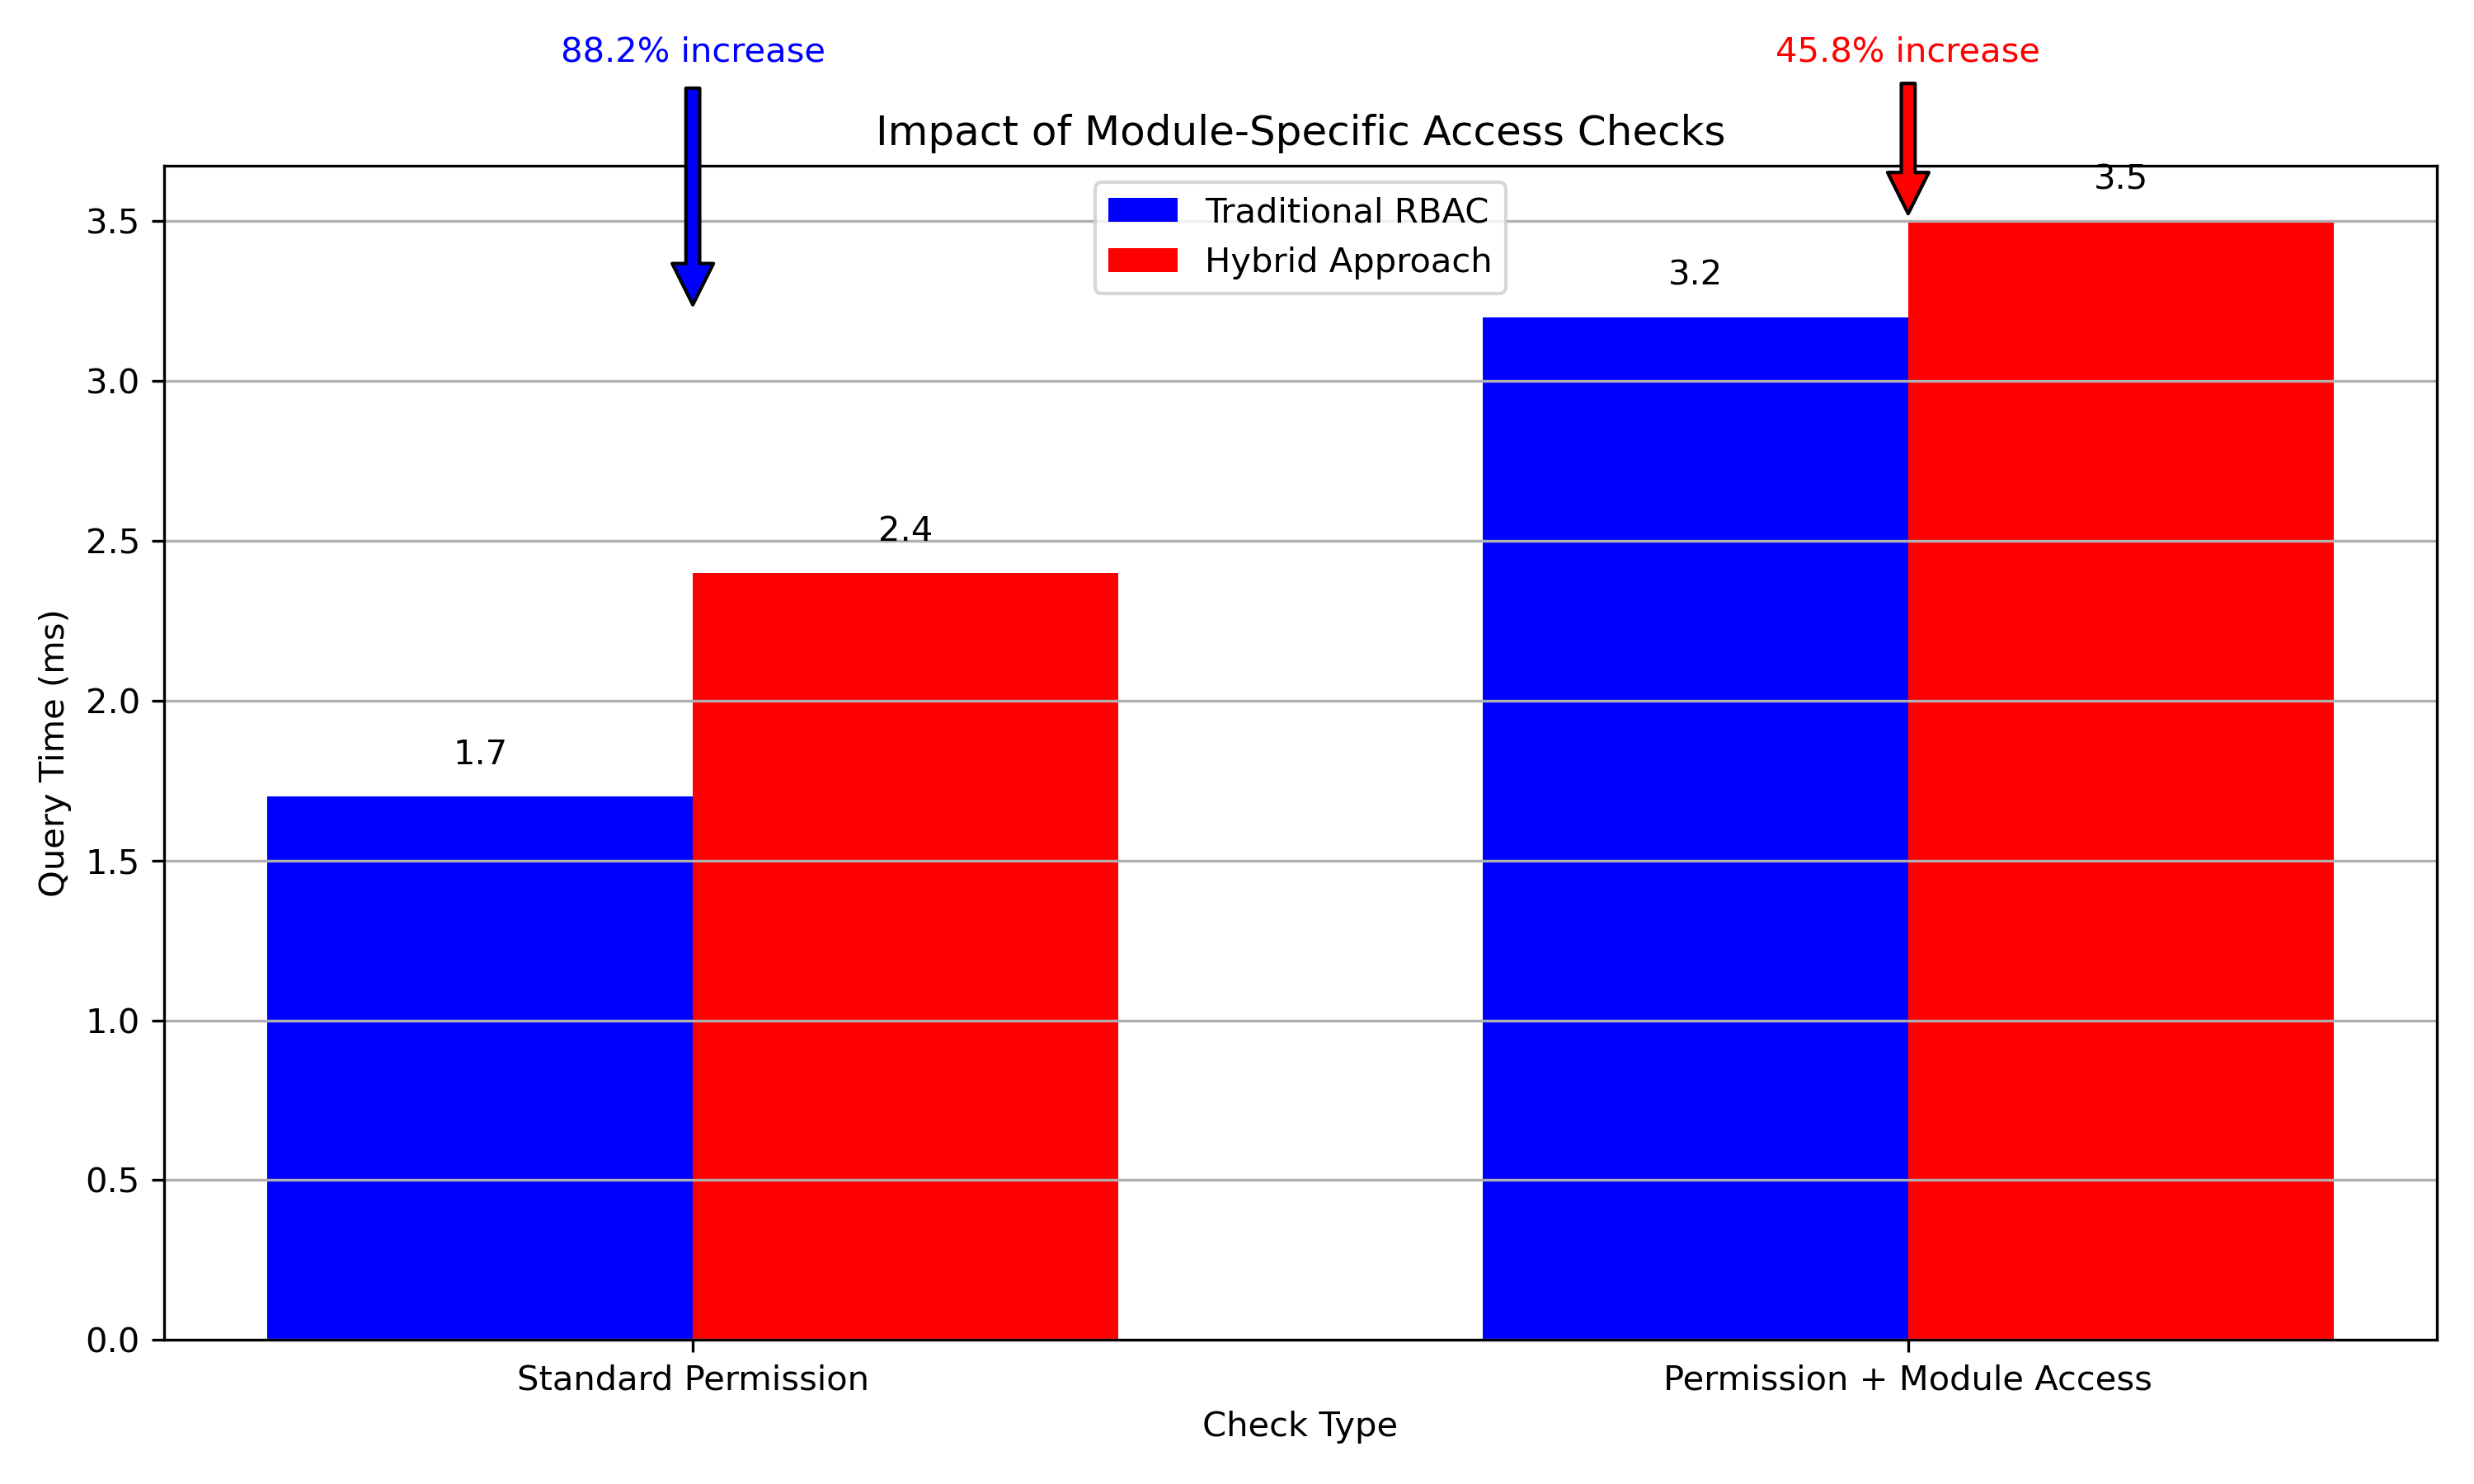
\includegraphics[width=0.8\textwidth]{figures/module_access_impact.png}
    \caption{Impact of Module-Specific Access Checks}
    \label{fig:module-access-impact}
\end{figure}

The performance analysis reveals that adding module-specific access verification introduces an 88.2\% overhead for the traditional role-based approach (increasing from 1.7ms to 3.2ms) and a 45.8\% overhead for the hybrid approach (increasing from 2.4ms to 3.5ms). Despite the performance overhead, both approaches maintain acceptable performance for interactive operations, with response times below 4ms for individual permission checks, confirming that the implemented module-specific access control provides the required access granularity without introducing prohibitive performance penalties.

\subsection{Release Management Validation}
\label{subsec:release-management-validation}

Release management testing evaluated the phase-based versioning approach that forms the foundation of the \ac{VMAP} system. Testing focused on four key aspects: phase sequence validation, phase transition operations, freeze functionality, and phase comparison. Phase sequence validation confirmed that the system correctly enforced the defined sequence of development phases with successful validation of each phase transition, essential for maintaining the structured development workflow described by Broy \cite{broy2006challenges} for automotive software development.

Phase transition testing verified that parameter configurations were correctly copied between phases with complete preservation of parameter-variant-segment relationships. Table \ref{tab:phase-transition-results} shows the test data revealing interesting patterns in development intensity across phases.

\begin{table}[h]
\centering
\caption{Phase Transition Test Results}
\label{tab:phase-transition-results}
\begin{tabular}{|l|c|c|p{2cm}|p{2cm}|c|}
\hline
\textbf{Transition Type} & \textbf{Variants} & \textbf{Segments} & \textbf{Added Variants} & \textbf{Added Segments} & \textbf{Time} \\
\hline
\multicolumn{6}{|c|}{\textbf{Baseline Dataset}} \\
\hline
Phase1 & 188 & 28,776 & - & - & - \\
\hline
Phase1 → Phase2 & 188 & 28,776 & 90 & 14,104 & 2.51s \\
\hline
Phase2 → Phase3 & 278 & 42,880 & 0 & 0 & 2.96s \\
\hline
Phase3 → Phase4 & 278 & 42,880 & 0 & 0 & 2.97s \\
\hline
\multicolumn{6}{|c|}{\textbf{Full Dataset}} \\
\hline
Phase1 & 830 & 167,990 & - & - & - \\
\hline
Phase1 → Phase2 & 830 & 167,990 & 170 & 41,113 & 12.39s \\
\hline
Phase2 → Phase3 & 1,000 & 209,103 & 0 & 0 & 12.87s \\
\hline
Phase3 → Phase4 & 1,000 & 209,103 & 0 & 0 & 12.89 \\
\hline
\end{tabular}
\end{table}

The test results reveal a significant pattern in development intensity across phases, consistent with Staron's observations \cite{staron2021automotive} regarding automotive software development cycles. The data demonstrates that the majority of parameter configurations occur during Phase1, with substantial additions in Phase2, while Phase3 and Phase4 typically involve refinement and validation rather than introducing new parameters or variants. This concentration of development activity in early phases aligns with the V-model approach common in automotive software development \cite{pretschner2007software}.

Phase transition performance characteristics showed only modest increases in execution time despite growing data volumes across phases. For the baseline dataset, transition times increased from 2.51s to approximately 3 seconds, demonstrating efficient scaling. Comparing baseline to full dataset transitions reveals transition times increasing to approximately 13 seconds, representing a sublinear scaling factor of approximately 4.3x for a dataset size increase of 5.6x.

Phase freezing functionality was validated through test cases targeting both database-level constraints and service-layer restrictions. The system successfully prevented modification attempts while maintaining appropriate read access, implementing the controlled milestone management required for regulated development environments as described by Staron \cite{staron2021automotive}.

\subsection{Variant Management Validation}
\label{subsec:variant-management-validation}

Variant management validation focused on assessing the system's capabilities for handling parameter customization through variants and segments. Testing employed an approach covering variant creation and segment modification workflows, using both the baseline dataset (188 variants, 28,776 segments) and the production-scale dataset (830 variants, 167,990 segments) to analyze functionality and performance under varying data volumes.

Variant creation testing verified proper implementation of domain constraints as defined in the conceptual architecture. Test cases included validation of unique name constraints within \acp{PID}, verification of proper code rule storage, and confirmation of correct relationship establishment between variants and their parent \acp{PID}. All test cases passed successfully for both scalar and complex parameters, with constraint enforcement consistently preventing invalid operations. As Vileikis \cite{vileikishacking} notes, constraint-based validation provides a robust foundation for maintaining data integrity in complex relational systems.

Performance analysis of variant operations revealed consistent response times across different variant complexities. Table \ref{tab:variant-operation-performance} details performance measurements for key variant operations under different data volumes.

\begin{table}[h]
\centering
\caption{Variant Operation Performance Metrics}
\label{tab:variant-operation-performance}
\begin{tabular}{|l|c|c|c|}
\hline
\textbf{Operation} & \textbf{Baseline Dataset} & \textbf{Production Dataset} & \textbf{Scaling Factor} \\
\hline
Variant Creation & 53ms & 55ms & 1.03x \\
\hline
Variant Update & 86ms & 124ms & 1.44x \\
\hline
Variant Retrieval & 45ms & 72ms & 1.60x \\
\hline
Variant Listing (per PID) & 38ms & 68ms & 1.79x \\
\hline
\end{tabular}
\end{table}

The observed scaling characteristics validate the effectiveness of the database schema design and indexing strategy described in Section \ref{sec:query-optimization}. The relatively small increase in execution time despite a 5x increase in data volume suggests efficient handling of larger datasets, with all operations remaining well under the 200ms threshold for interactive operations.

Segment modification testing employed a systematic approach covering one-dimensional arrays, two-dimensional matrices, and three-dimensional parameter representations. The database schema design proved effective for managing these complex data structures, with robust constraint enforcement correctly rejecting segment modifications with invalid dimension indices. Performance analysis for segment operations showed moderate scaling across different dataset sizes, with scaling factors ranging from 1.46x to 1.81x, validating the efficiency of the database schema design described in Section \ref{sec:entity-relationship-model}.

\section{Performance Analysis}
\label{sec:performance-analysis}

Beyond functional validation, performance analysis was conducted to assess the system's efficiency and scalability under various operational conditions. This section presents the key findings related to query performance and data volume scaling.

\subsection{Query Performance Assessment}
\label{subsec:query-performance-assessment}

Query performance was evaluated for common database operations across different data volumes. Figure~\ref{fig:query-performance-comparison} presents performance measurements for key query types between the baseline dataset (20,000 parameters) and full dataset (100,000 parameters).

\begin{figure}[h]
    \centering
    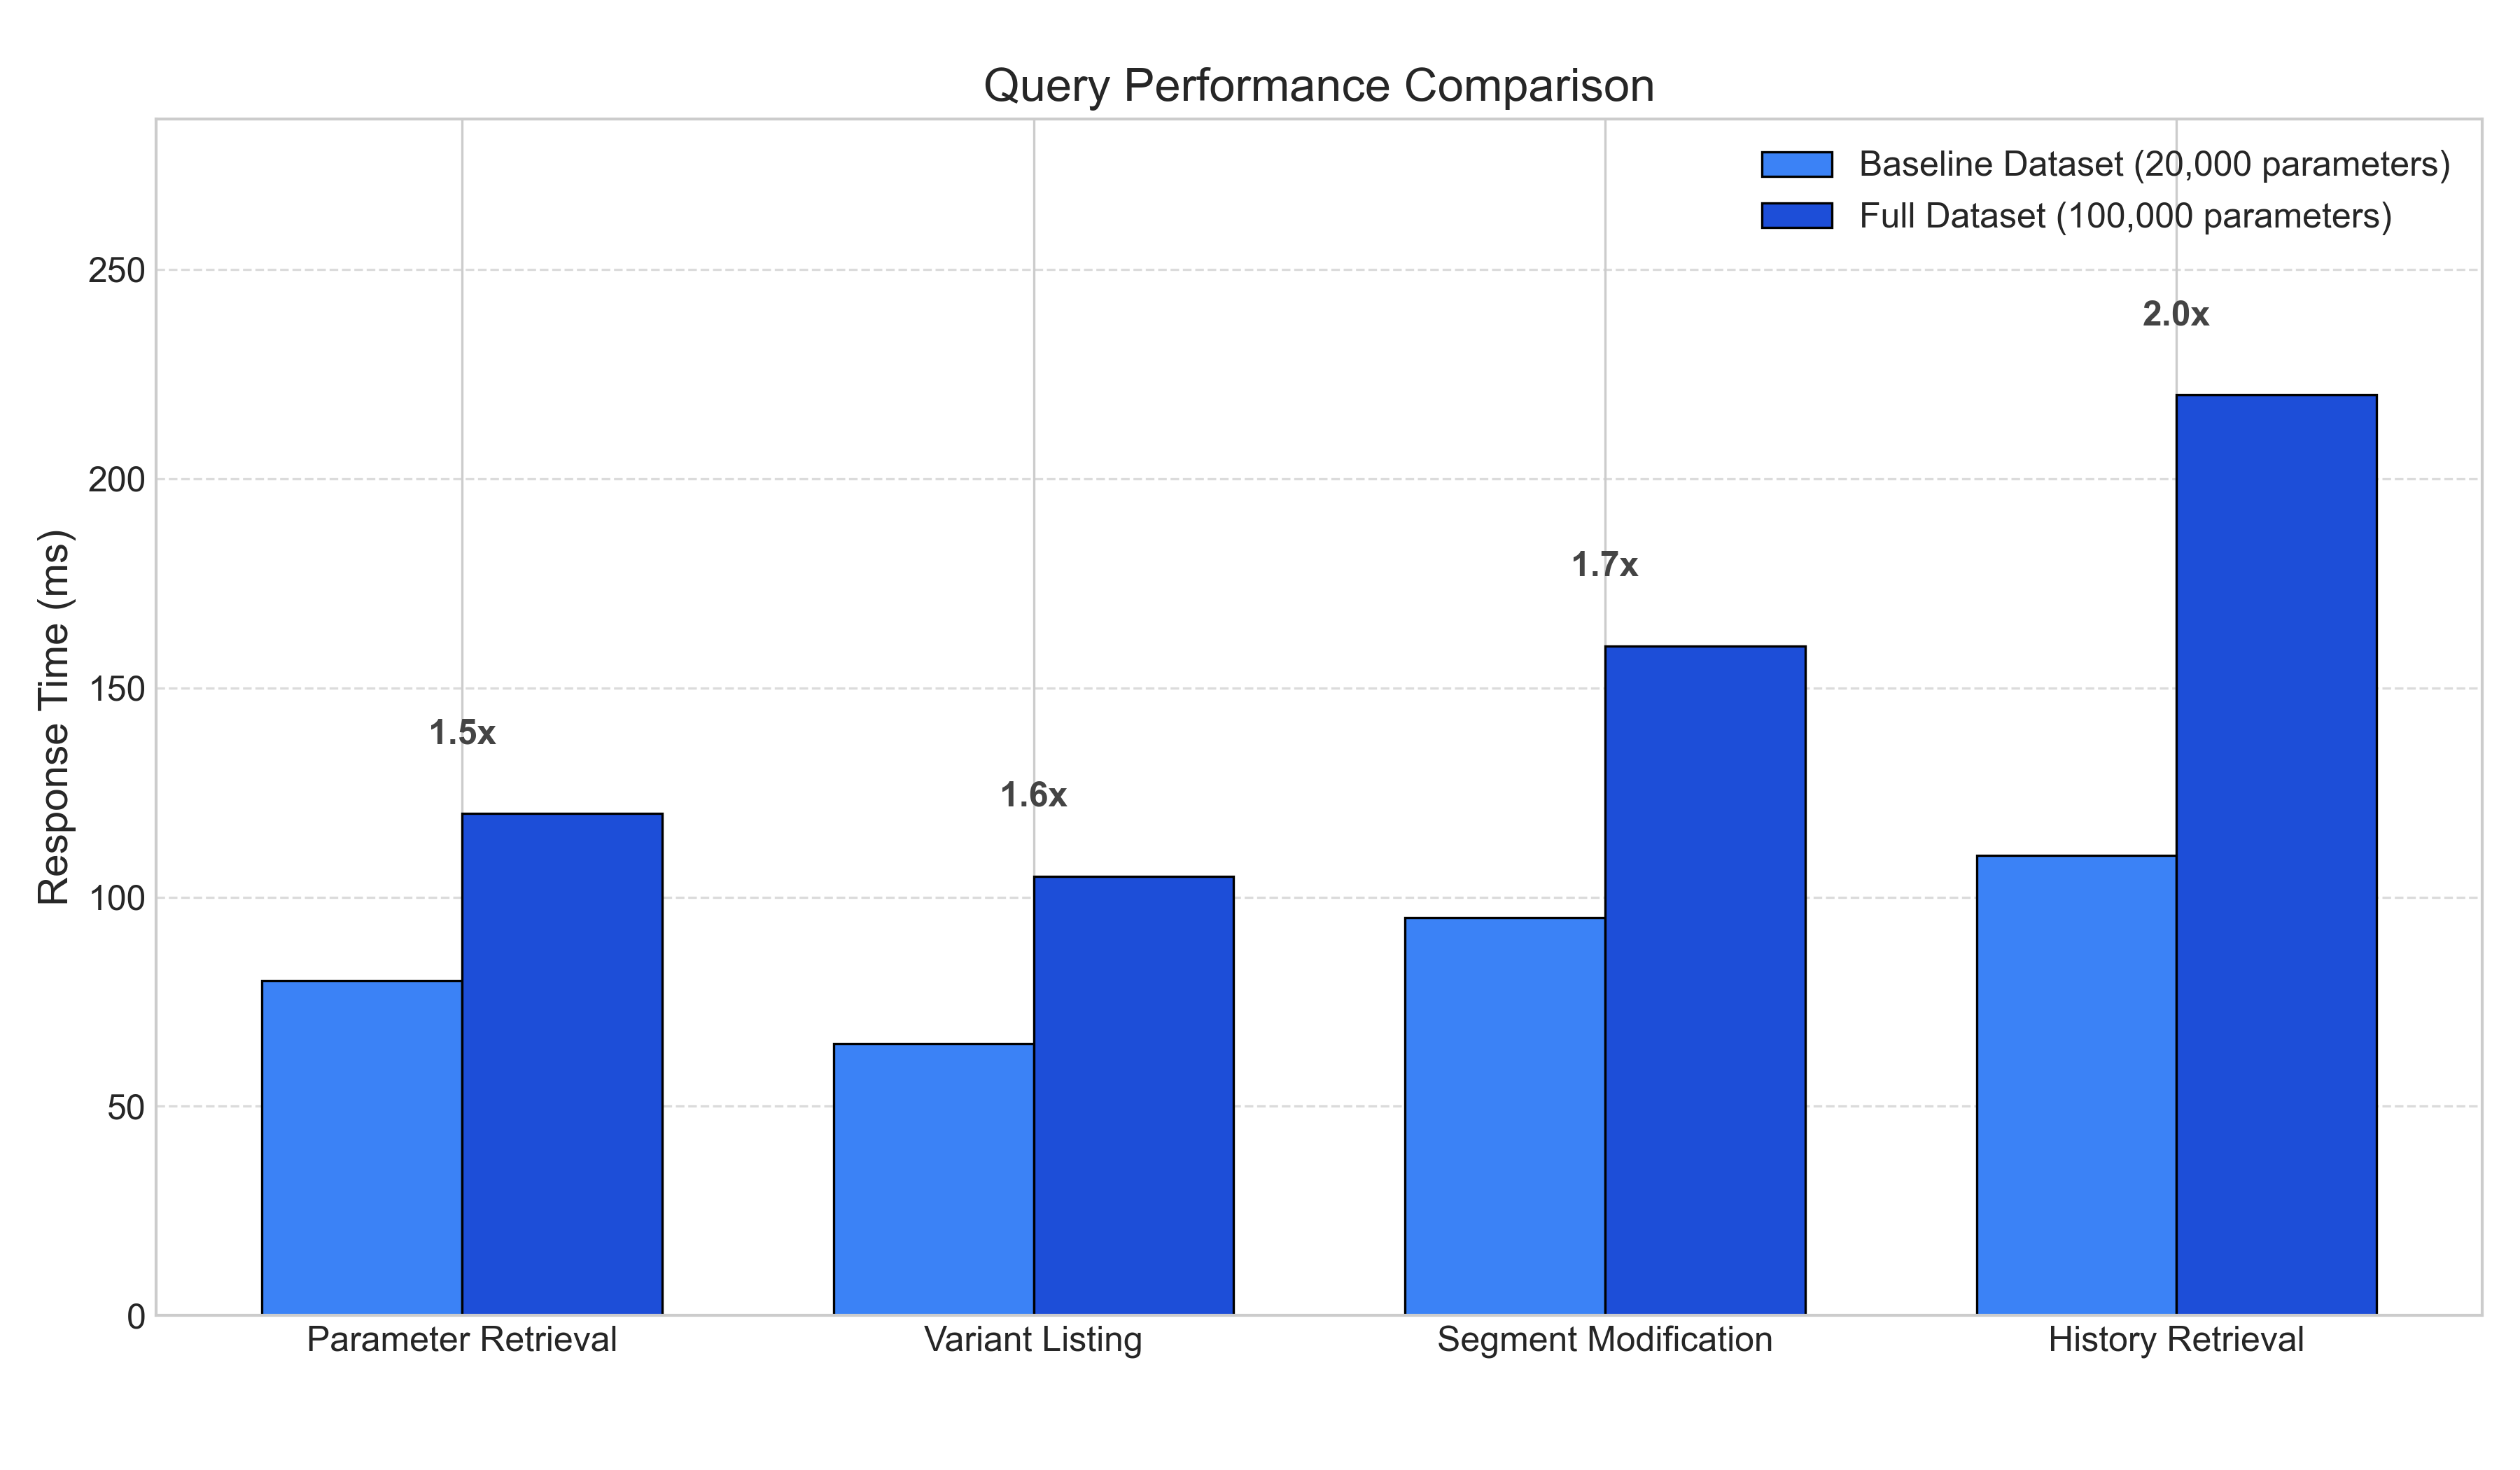
\includegraphics[width=0.8\textwidth]{figures/query_performance_comparison.png}
    \caption{Query Performance Comparison}
    \label{fig:query-performance-comparison}
\end{figure}

The performance analysis reveals that most common operations maintain reasonable performance with increasing data volumes. The system maintained interactive response times (below 200ms) for most operations even with the full dataset, ensuring a responsive user experience. Parameter retrieval operations showed a scaling factor of 1.5x when moving from the baseline to full dataset, while variant listing demonstrated a slightly higher factor of 1.6x. History retrieval operations exhibited the highest scaling factor among standard queries at 2.0x, reflecting the additional processing required when retrieving records from the substantially larger audit history tables.

The phase comparison operation demonstrated longer execution times and suboptimal scaling, with execution times increasing from 2.8s for the baseline dataset to 12.4s for the full dataset—a scaling factor of 4.4x. This operation exceeds the interactive response threshold for larger datasets, identifying it as a candidate for future optimization. The execution of queries with and without indexes demonstrated the critical importance of the indexing strategy, with response times increasing by factors of 6.5x to 21.8x without proper indexes.

\subsection{Indexing Strategy Performance Validation}
\label{subsec:indexing-strategy-performance}

The indexing strategy described in Section \ref{sec:query-optimization} was validated through comprehensive performance measurements comparing query execution times with and without strategic indexes. Figure \ref{fig:index-performance-comparison} presents the performance comparison across five critical query patterns that represent the dominant access patterns in automotive parameter management workflows.

\begin{figure}[h]
    \centering
    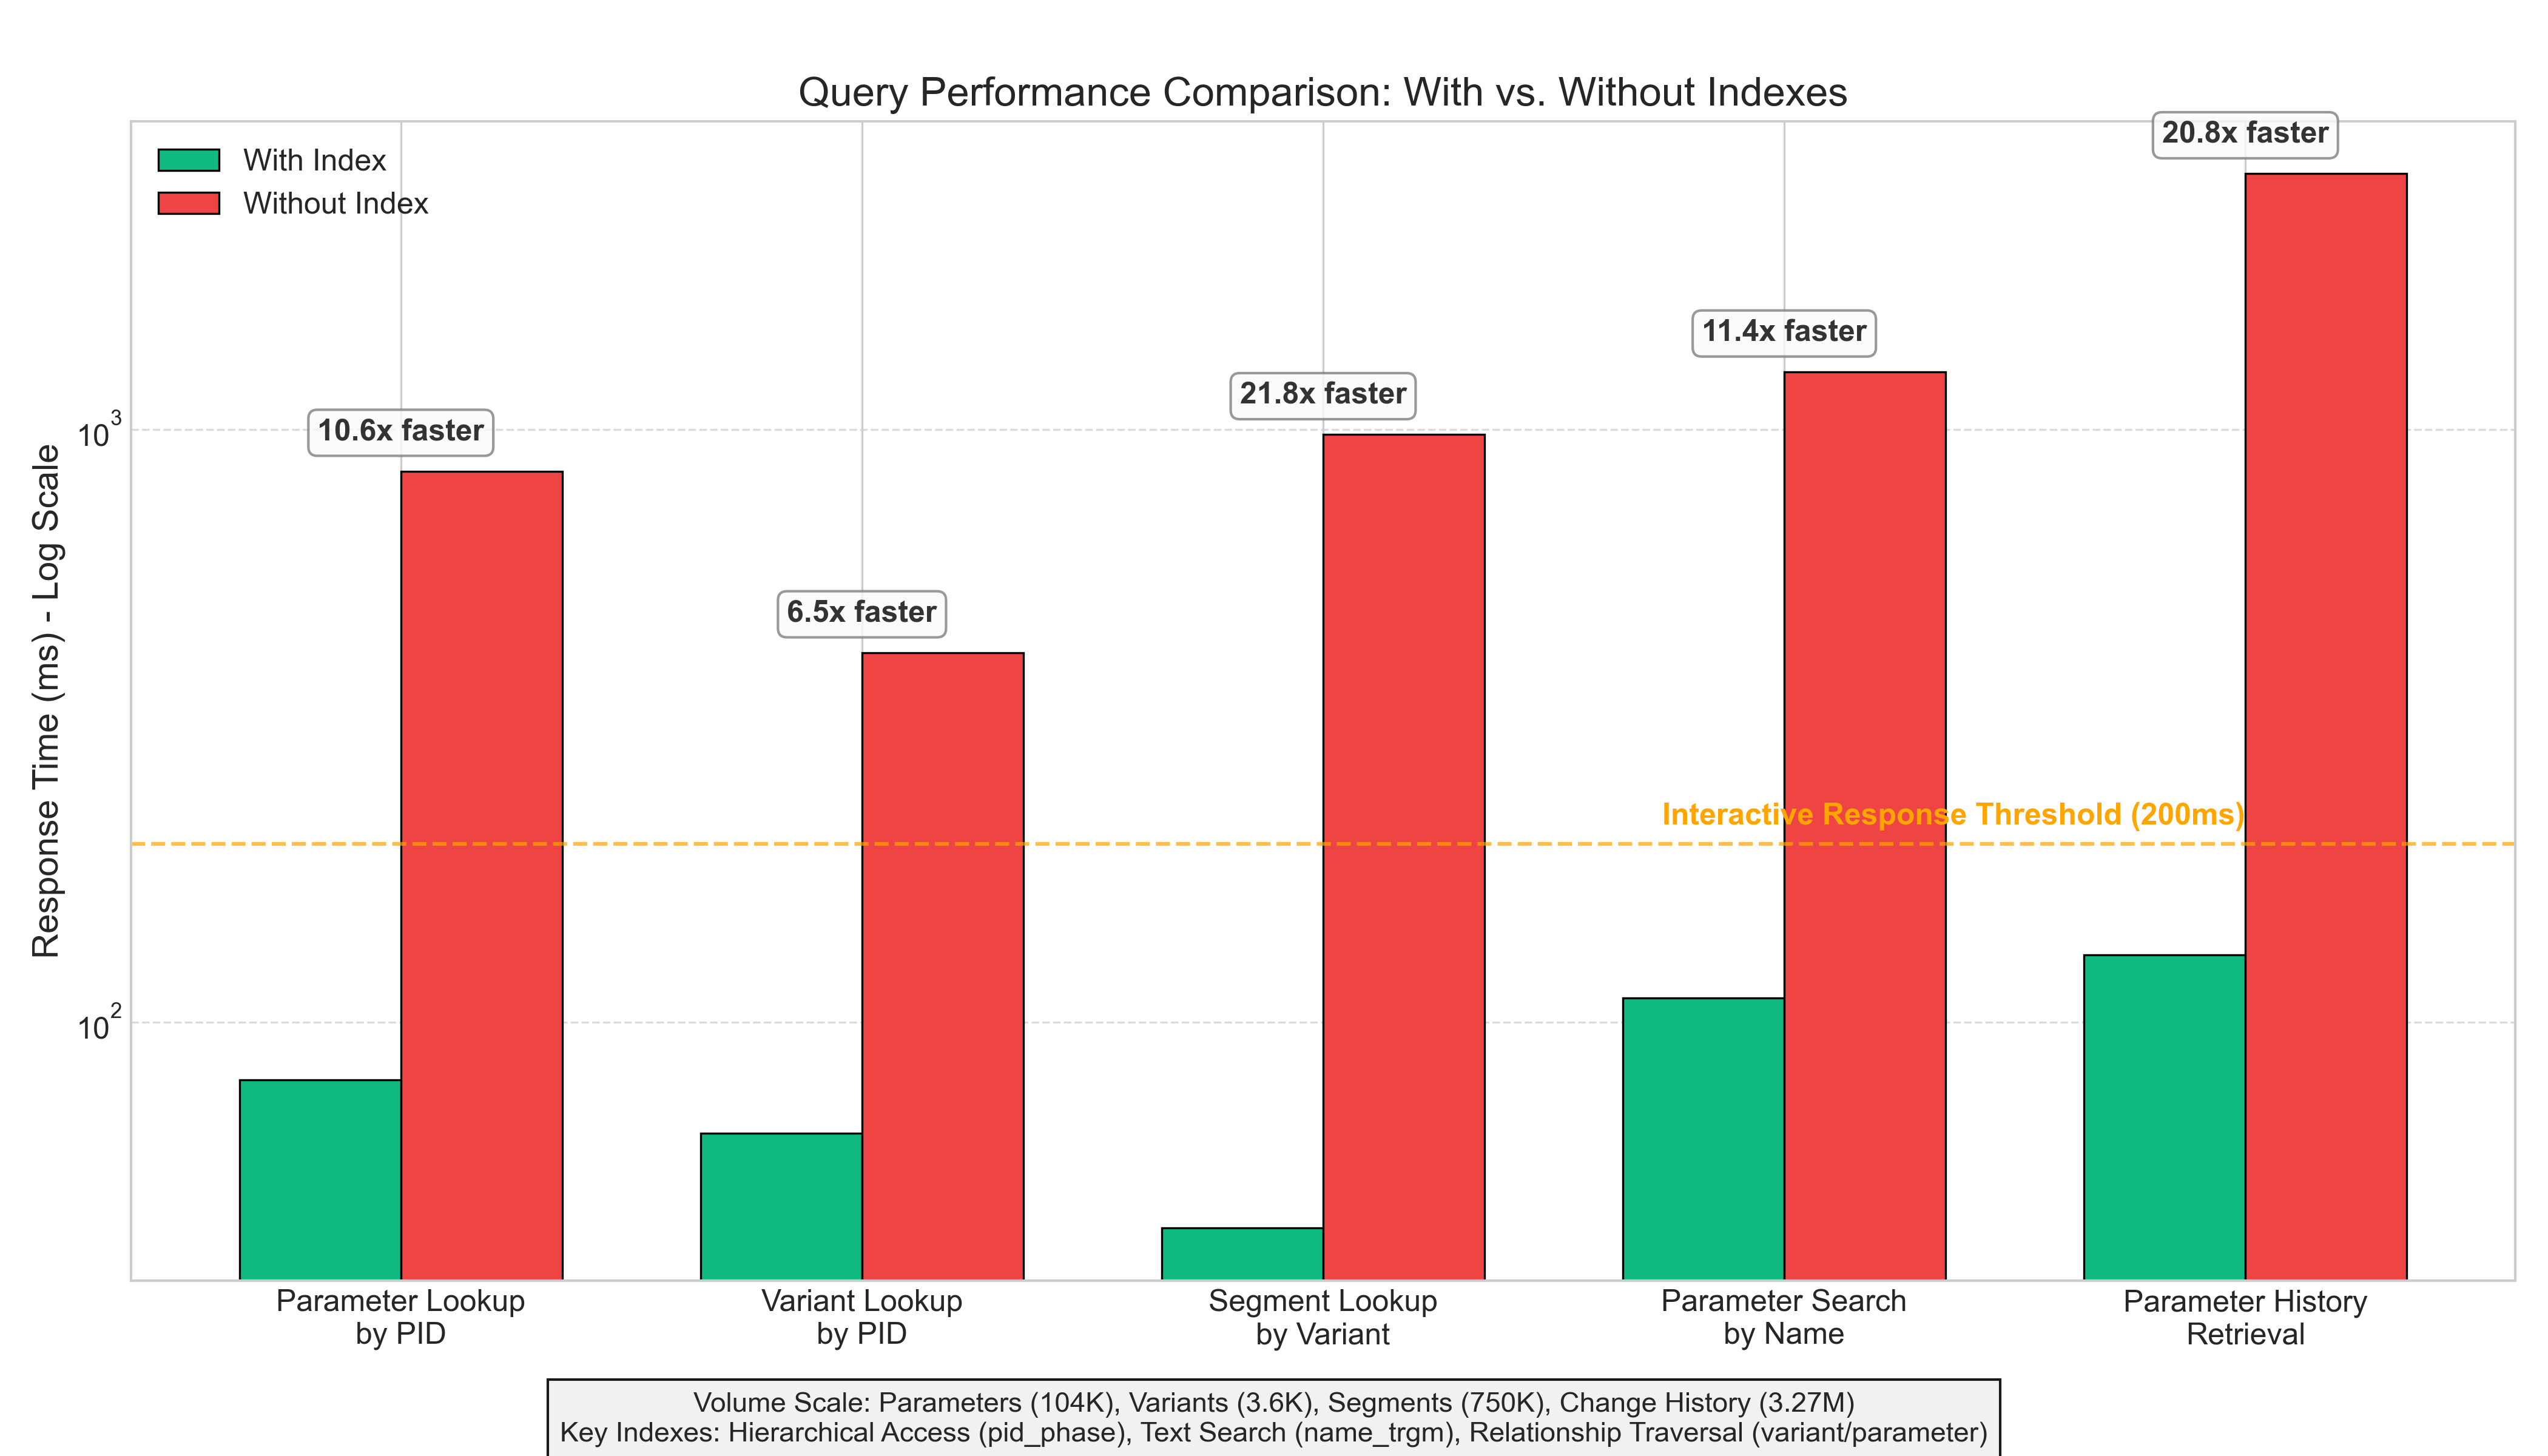
\includegraphics[width=0.95\textwidth]{figures/index_performance_comparison.png}
    \caption{Query Performance Comparison: With vs. Without Indexes}
    \label{fig:index-performance-comparison}
\end{figure}

The performance evaluation demonstrates the critical importance of the implemented indexing strategy for maintaining interactive response times in production environments. Parameter lookup operations by PID achieved a 10.6x performance improvement, reducing response times from 850ms to 80ms through the \texttt{idx\_parameters\_\allowbreak pid\_\allowbreak phase} composite index. Variant lookup operations showed a 6.5x improvement, with response times decreasing from 420ms to 65ms using the same hierarchical indexing approach. The most dramatic improvement was observed in segment lookup operations, which achieved a 21.8x speedup from 980ms to 45ms through the \texttt{idx\_segments\_variant} index, reflecting the efficiency of direct relationship traversal compared to sequential scanning.

Text-based parameter search operations, enabled by PostgreSQL's trigram indexes, demonstrated an 11.4x performance improvement from 1,250ms to 110ms. This capability is particularly valuable for engineering workflows where parameters are often located through partial name matching rather than exact hierarchical navigation. Parameter history retrieval, which accesses the extensive change history tables containing over 3.2 million records, showed the most substantial absolute improvement with a 20.8x speedup from 2,700ms to 130ms, validating the effectiveness of the audit system indexing strategy described in Section \ref{sec:audit-system}.

All indexed operations maintained response times well below the 200ms interactive response threshold, ensuring that the system provides a responsive user experience even with production-scale datasets containing over 100,000 parameters. The performance improvements validate the strategic indexing decisions made during implementation, particularly the use of composite indexes for hierarchical navigation and specialized trigram indexes for text-based searching. These results demonstrate that the database design successfully addresses the performance requirements of automotive parameter management while maintaining the comprehensive audit capabilities essential for regulatory compliance.

\subsection{Variant Operation Performance}
\label{subsec:variant-operation-performance}

Variant operation performance was assessed across different data volumes to evaluate the system's handling of core parameter customization workflows. Figure~\ref{fig:variant-performance} illustrates the performance of variant operations under different data volumes.

\begin{figure}[h]
    \centering
    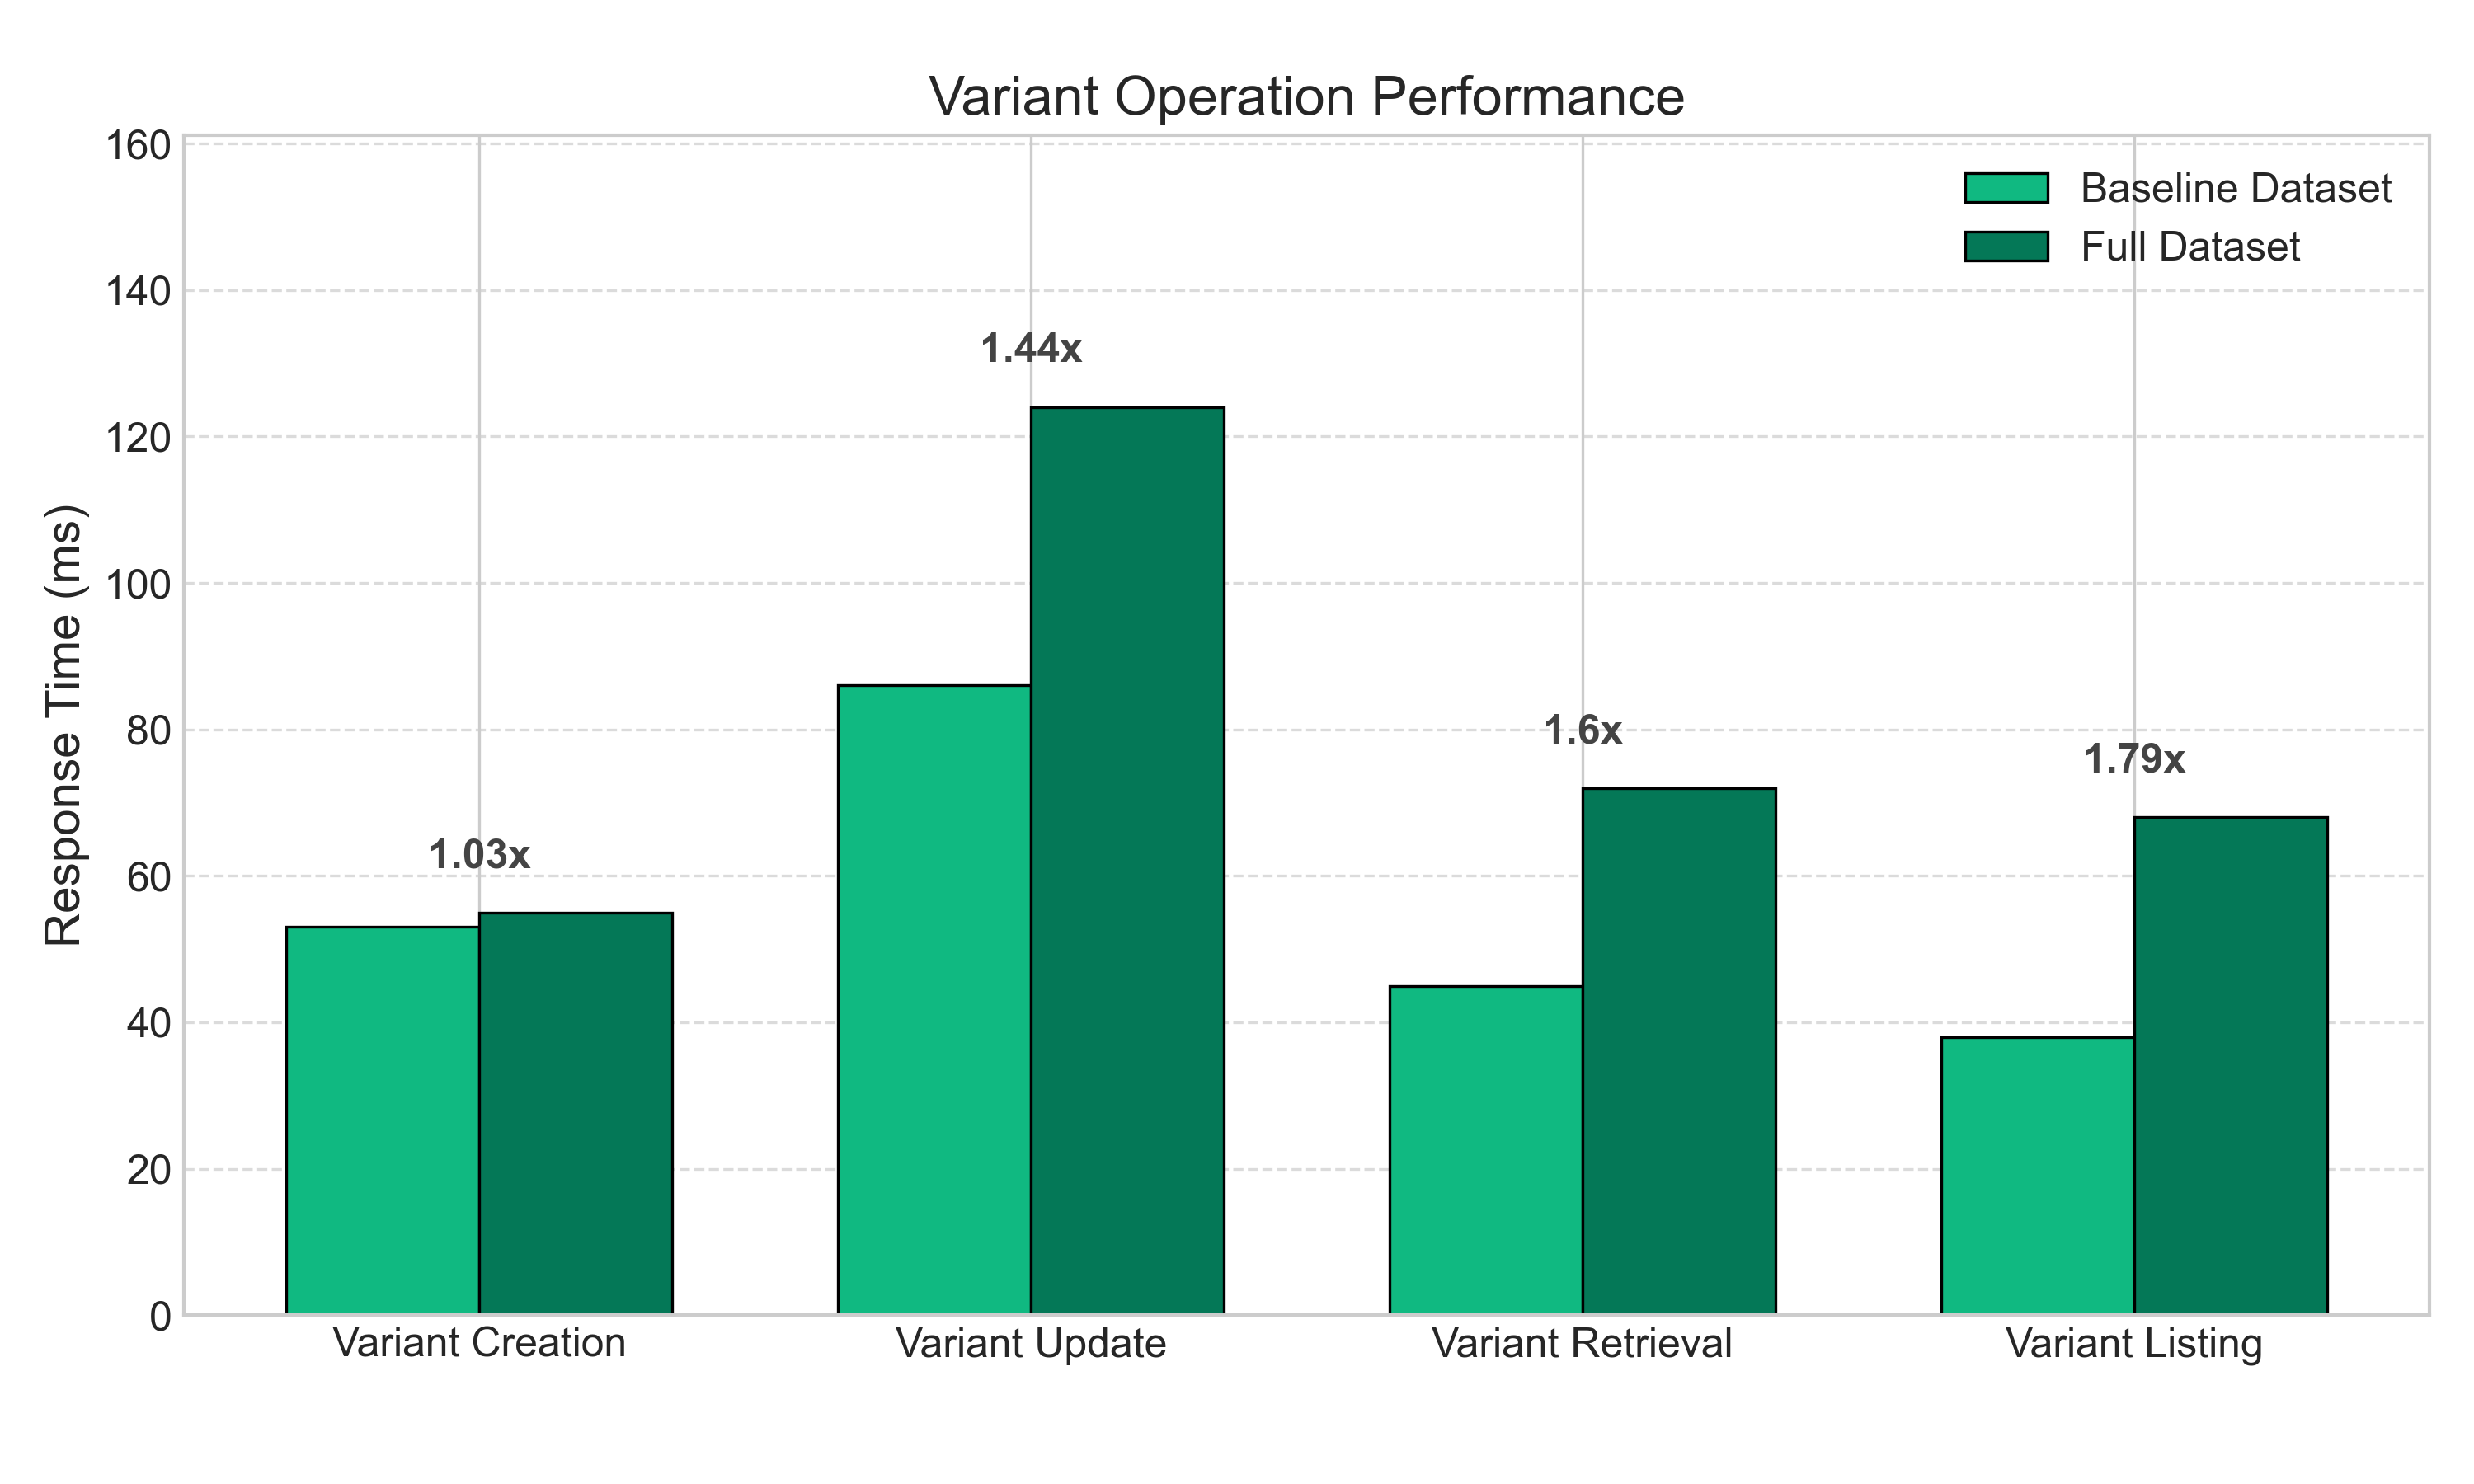
\includegraphics[width=0.8\textwidth]{figures/variant_performance.png}
    \caption{Variant Operation Performance}
    \label{fig:variant-performance}
\end{figure}

The analysis reveals consistent response times across different operation types, with scaling factors ranging from 1.03x for variant creation to 1.79x for variant listing when comparing baseline and full datasets. Variant creation operations demonstrated excellent scaling characteristics (1.03x), showing minimal performance impact despite the five-fold increase in dataset size. This efficiency can be attributed to the well-designed primary key and constraint implementation, allowing new records to be inserted with minimal overhead regardless of existing data volume. The average scaling factor across all variant operations was approximately 1.47x, indicating that these operations scale efficiently with increasing data volumes, with all variant operations maintaining response times under 125ms for the full dataset.

\subsection{Storage Requirements Analysis}
\label{subsec:storage-requirements-analysis}

Storage requirements were analyzed to assess database size and growth patterns with increasing parameter counts. Figure~\ref{fig:storage-analysis} presents the storage allocation across different entity types for the full dataset.

\begin{figure}[h]
    \centering
    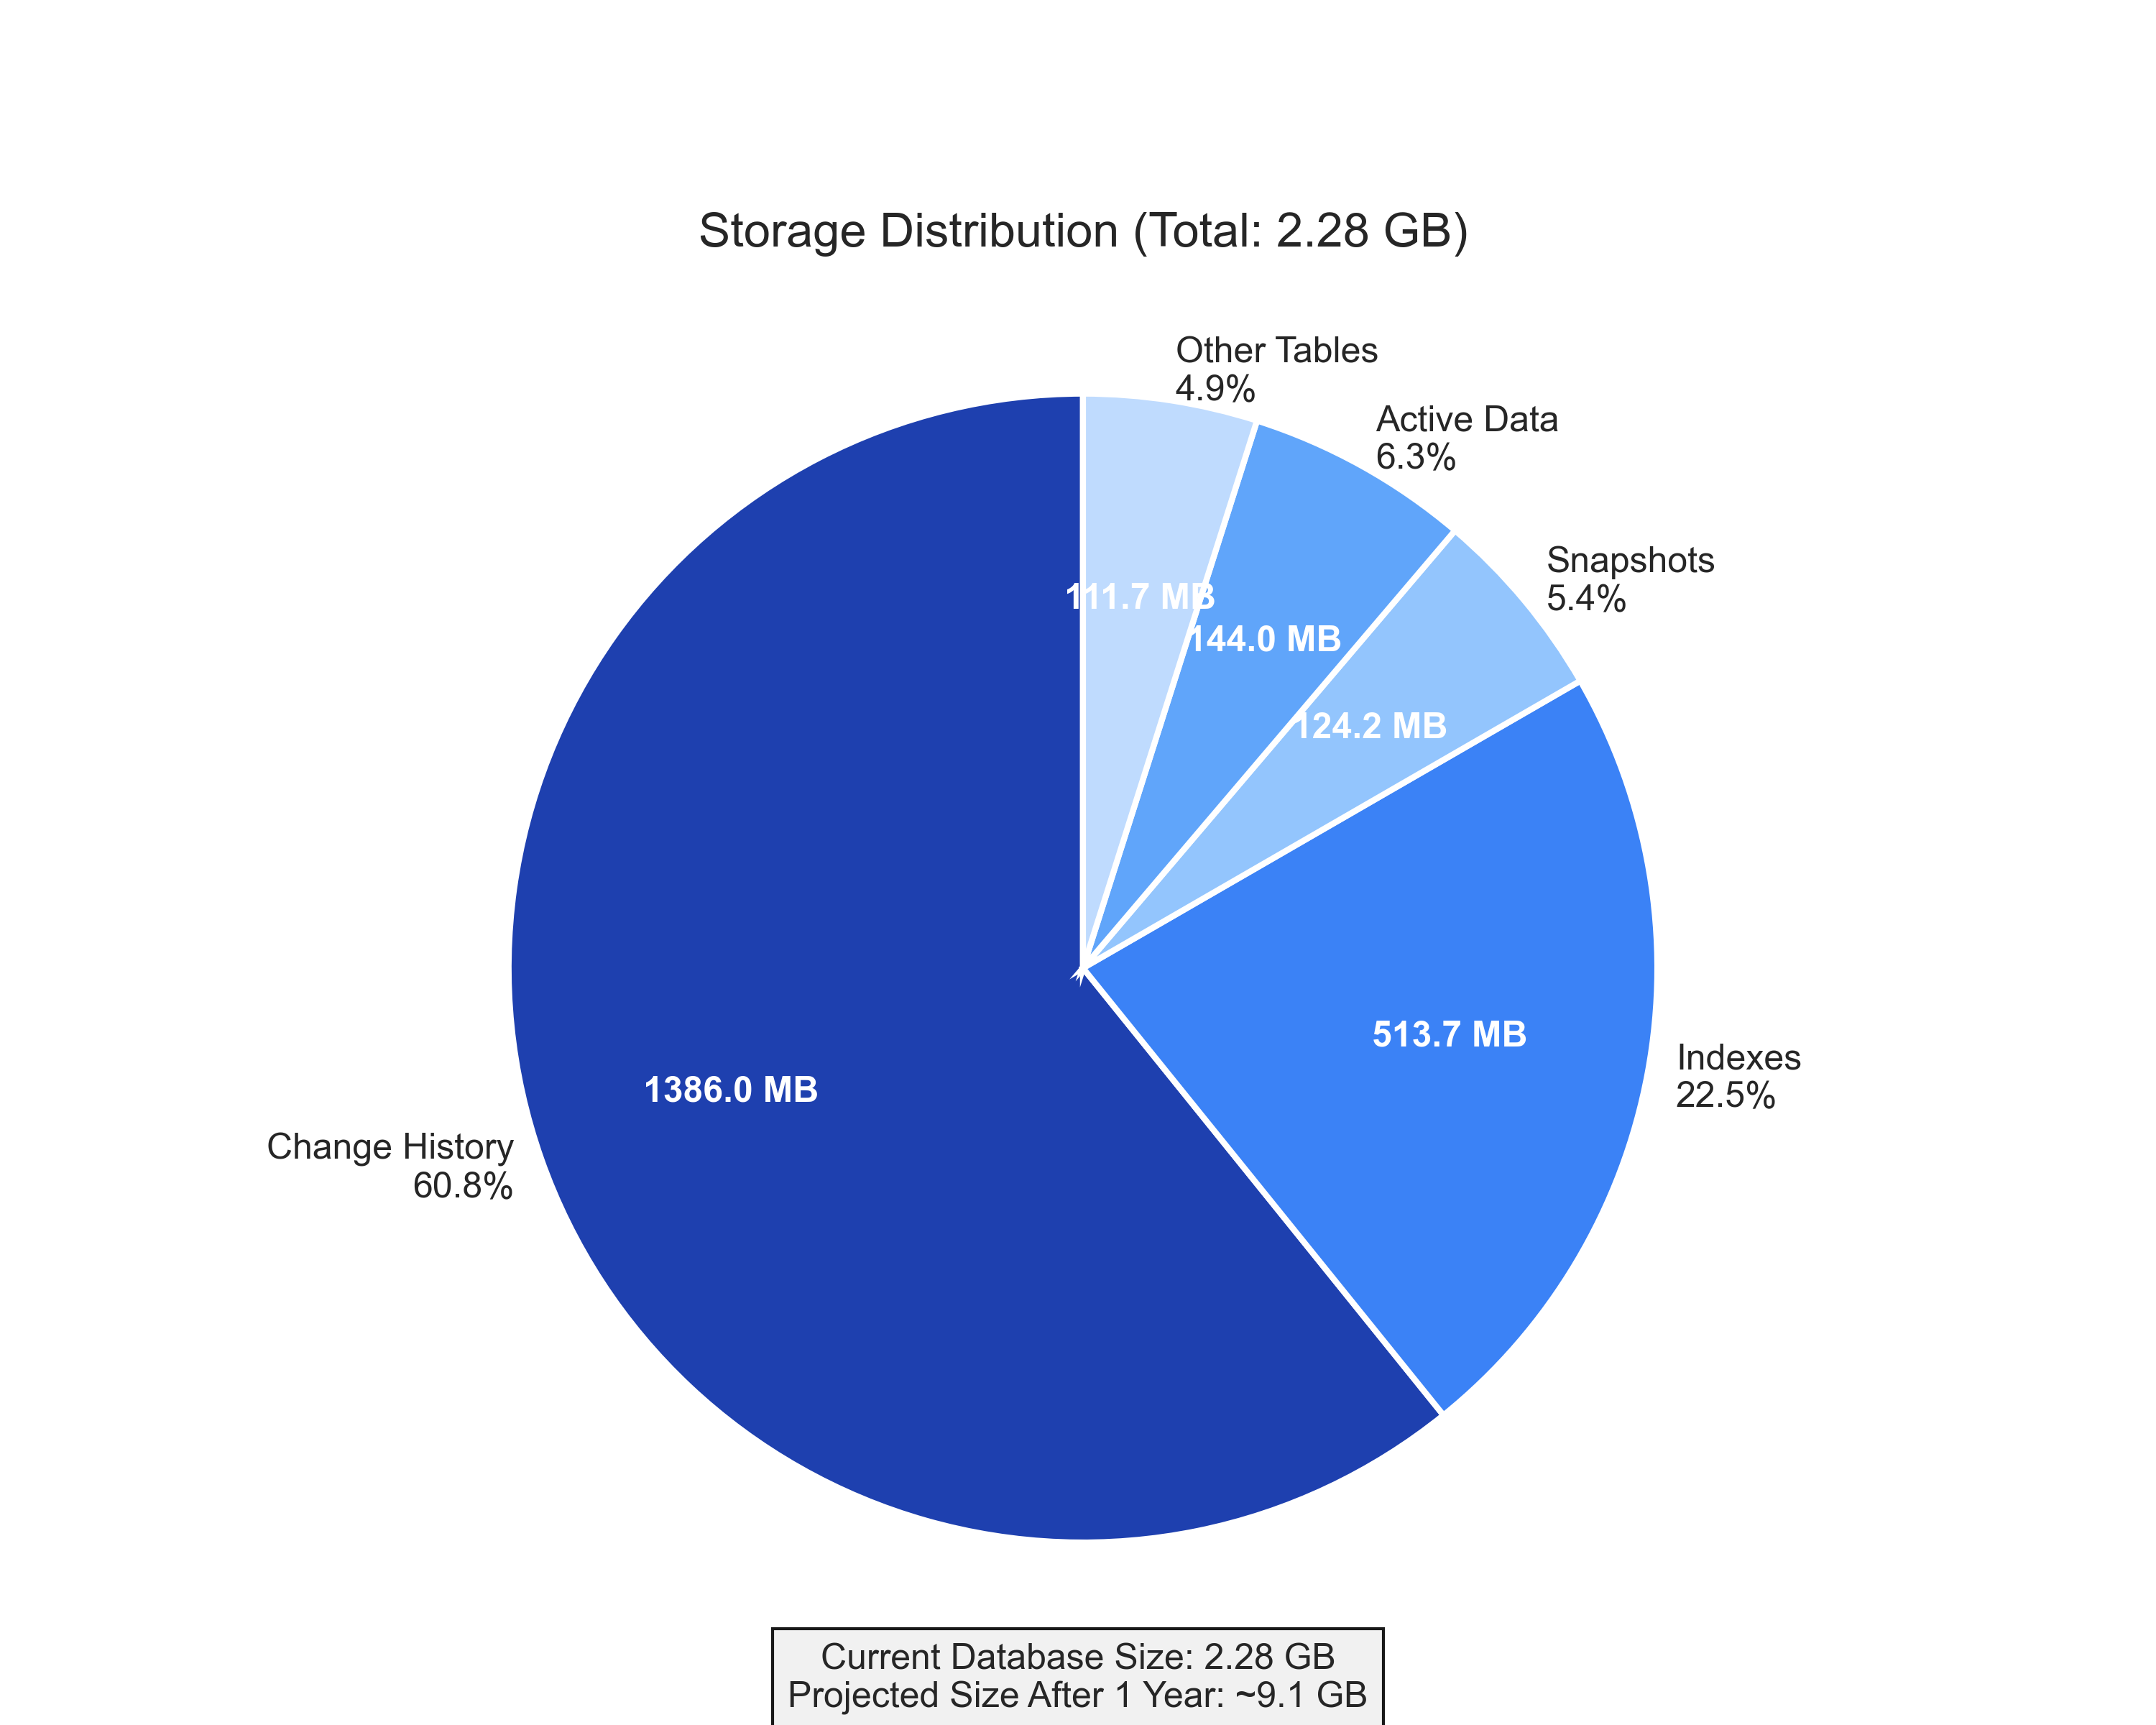
\includegraphics[width=0.8\textwidth]{figures/storage_distribution.png}
    \caption{Storage Distribution by Entity Type}
    \label{fig:storage-analysis}
\end{figure}

The analysis reveals that the change history table dominates the database storage allocation, accounting for approximately 60.8\% of the total database size. This distribution significantly exceeds the storage requirements of the current data state, aligning with Bhattacherjee's observations~\cite{bhattacherjee2015principles} regarding versioning and audit systems. While there are only 3,617 variants in the current state, the system maintains over 3.2 million change history records, reflecting the comprehensive auditing approach implemented in the system.

\begin{table}[h]
\centering
\caption{Storage Requirements Analysis}
\label{tab:storage-requirements}
\begin{tabular}{|l|r|r|}
\hline
\textbf{Entity Type} & \textbf{Record Count} & \textbf{Storage Size (MB)} \\
\hline
Parameters & 104,428 & 43.0 \\
\hline
Variants & 3,617 & 1.0 \\
\hline
Segments & 750,009 & 100.0 \\
\hline
Change History & 3,270,511 & 1,386.0 \\
\hline
Documentation Snapshots & 7 & 0.1 \\
\hline
Snapshot Variants & 4,980 & 0.1 \\
\hline
Snapshot Segments & 1,007,940 & 124.0 \\
\hline
Other Tables & - & 111.7 \\
\hline
Indexes & - & 513.7 \\
\hline
\textbf{Total} & - & \textbf{2,279.6} \\
\hline
\end{tabular}
\end{table}

Despite having only 7 documentation snapshots, the system maintains over 1 million snapshot segments, exceeding the count of active segments. This indicates that documentation snapshots capture extensive parameter configurations at specific time points, creating substantial storage requirements for historical state preservation. The index structures consume approximately 22.5\% of the total storage, reflecting the sophisticated indexing strategy described in Section~\ref{sec:query-optimization}. While this represents significant overhead, it provides essential performance benefits for query operations.

The actual active data—parameters, variants, and segments—consumes only 6.3\% of the total database size, with the majority of storage dedicated to audit trails, snapshots, and indexes. This distribution aligns with the requirements for regulated development environments described by Staron~\cite{staron2021automotive}, where comprehensive traceability and historical record maintenance are essential for compliance and quality assurance.

\subsection{Versioning Approach Performance}
\label{subsec:versioning-approach-performance}

The performance characteristics of the phase-based parameter versioning approach selected in Chapter~\ref{chap:methodology} were evaluated against the alternative change-based approach. Figure~\ref{fig:versioning-approach-comparison} presents the performance comparison between the two approaches for parameter retrieval operations across different data volumes, along with the storage requirements for each approach.

\begin{figure}[h]
    \centering
    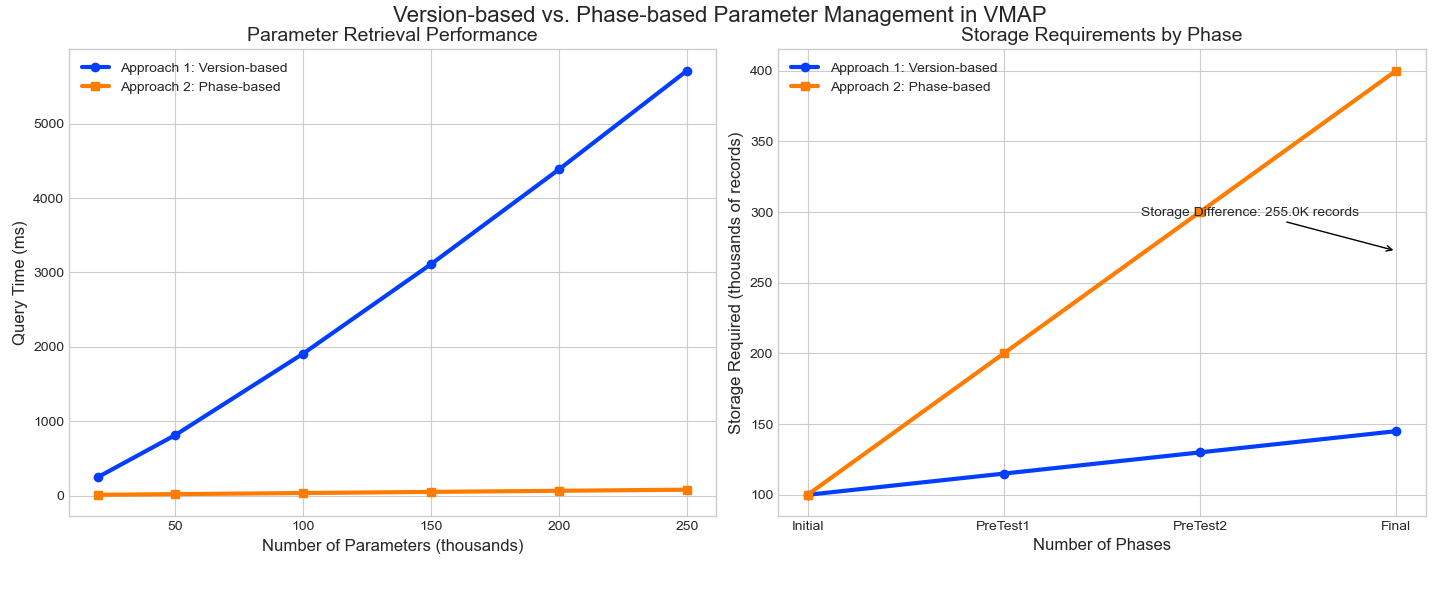
\includegraphics[width=0.8\textwidth]{figures/vmap_versioning_approaches_simplified.png}
    \caption{Version-based vs. Phase-based Parameter Management Comparison}
    \label{fig:versioning-approach-comparison}
\end{figure}

The performance analysis demonstrates that the phase-based approach offers better query performance, particularly as parameter counts increase. For the tested parameter counts, the phase-based approach remains below 100ms for parameter retrieval operations, while the version-based approach shows nonlinear growth with increasing parameter counts. The storage requirements analysis confirms that the phase-based approach consumes approximately 51\% higher storage requirements across all phases. However, this storage difference represents a reasonable tradeoff given the performance benefits for query operations, as noted by Bhattacherjee et al.~\cite{bhattacherjee2015principles}.

These findings validate the architectural decision to implement a phase-based versioning approach for the \ac{VMAP} system. While consuming more storage than a version-based approach, the phase model provides performance benefits, implementation simplicity, and alignment with domain concepts that outweigh the additional storage requirements.

\section{Integration Testing}
\label{sec:integration-testing}

Integration testing evaluated the system's interaction with external enterprise systems, focusing on Parameter Definition Database synchronization and Vehicle Configuration Database integration.

\subsection{Parameter Definition Database Synchronization}
\label{subsec:pdd-synchronization-testing}

Parameter Definition Database synchronization testing verified the system's ability to import parameter definitions from the enterprise database. Figure \ref{fig:pdd-sync-time} illustrates the synchronization time trends observed during testing.

\begin{figure}[h]
    \centering
    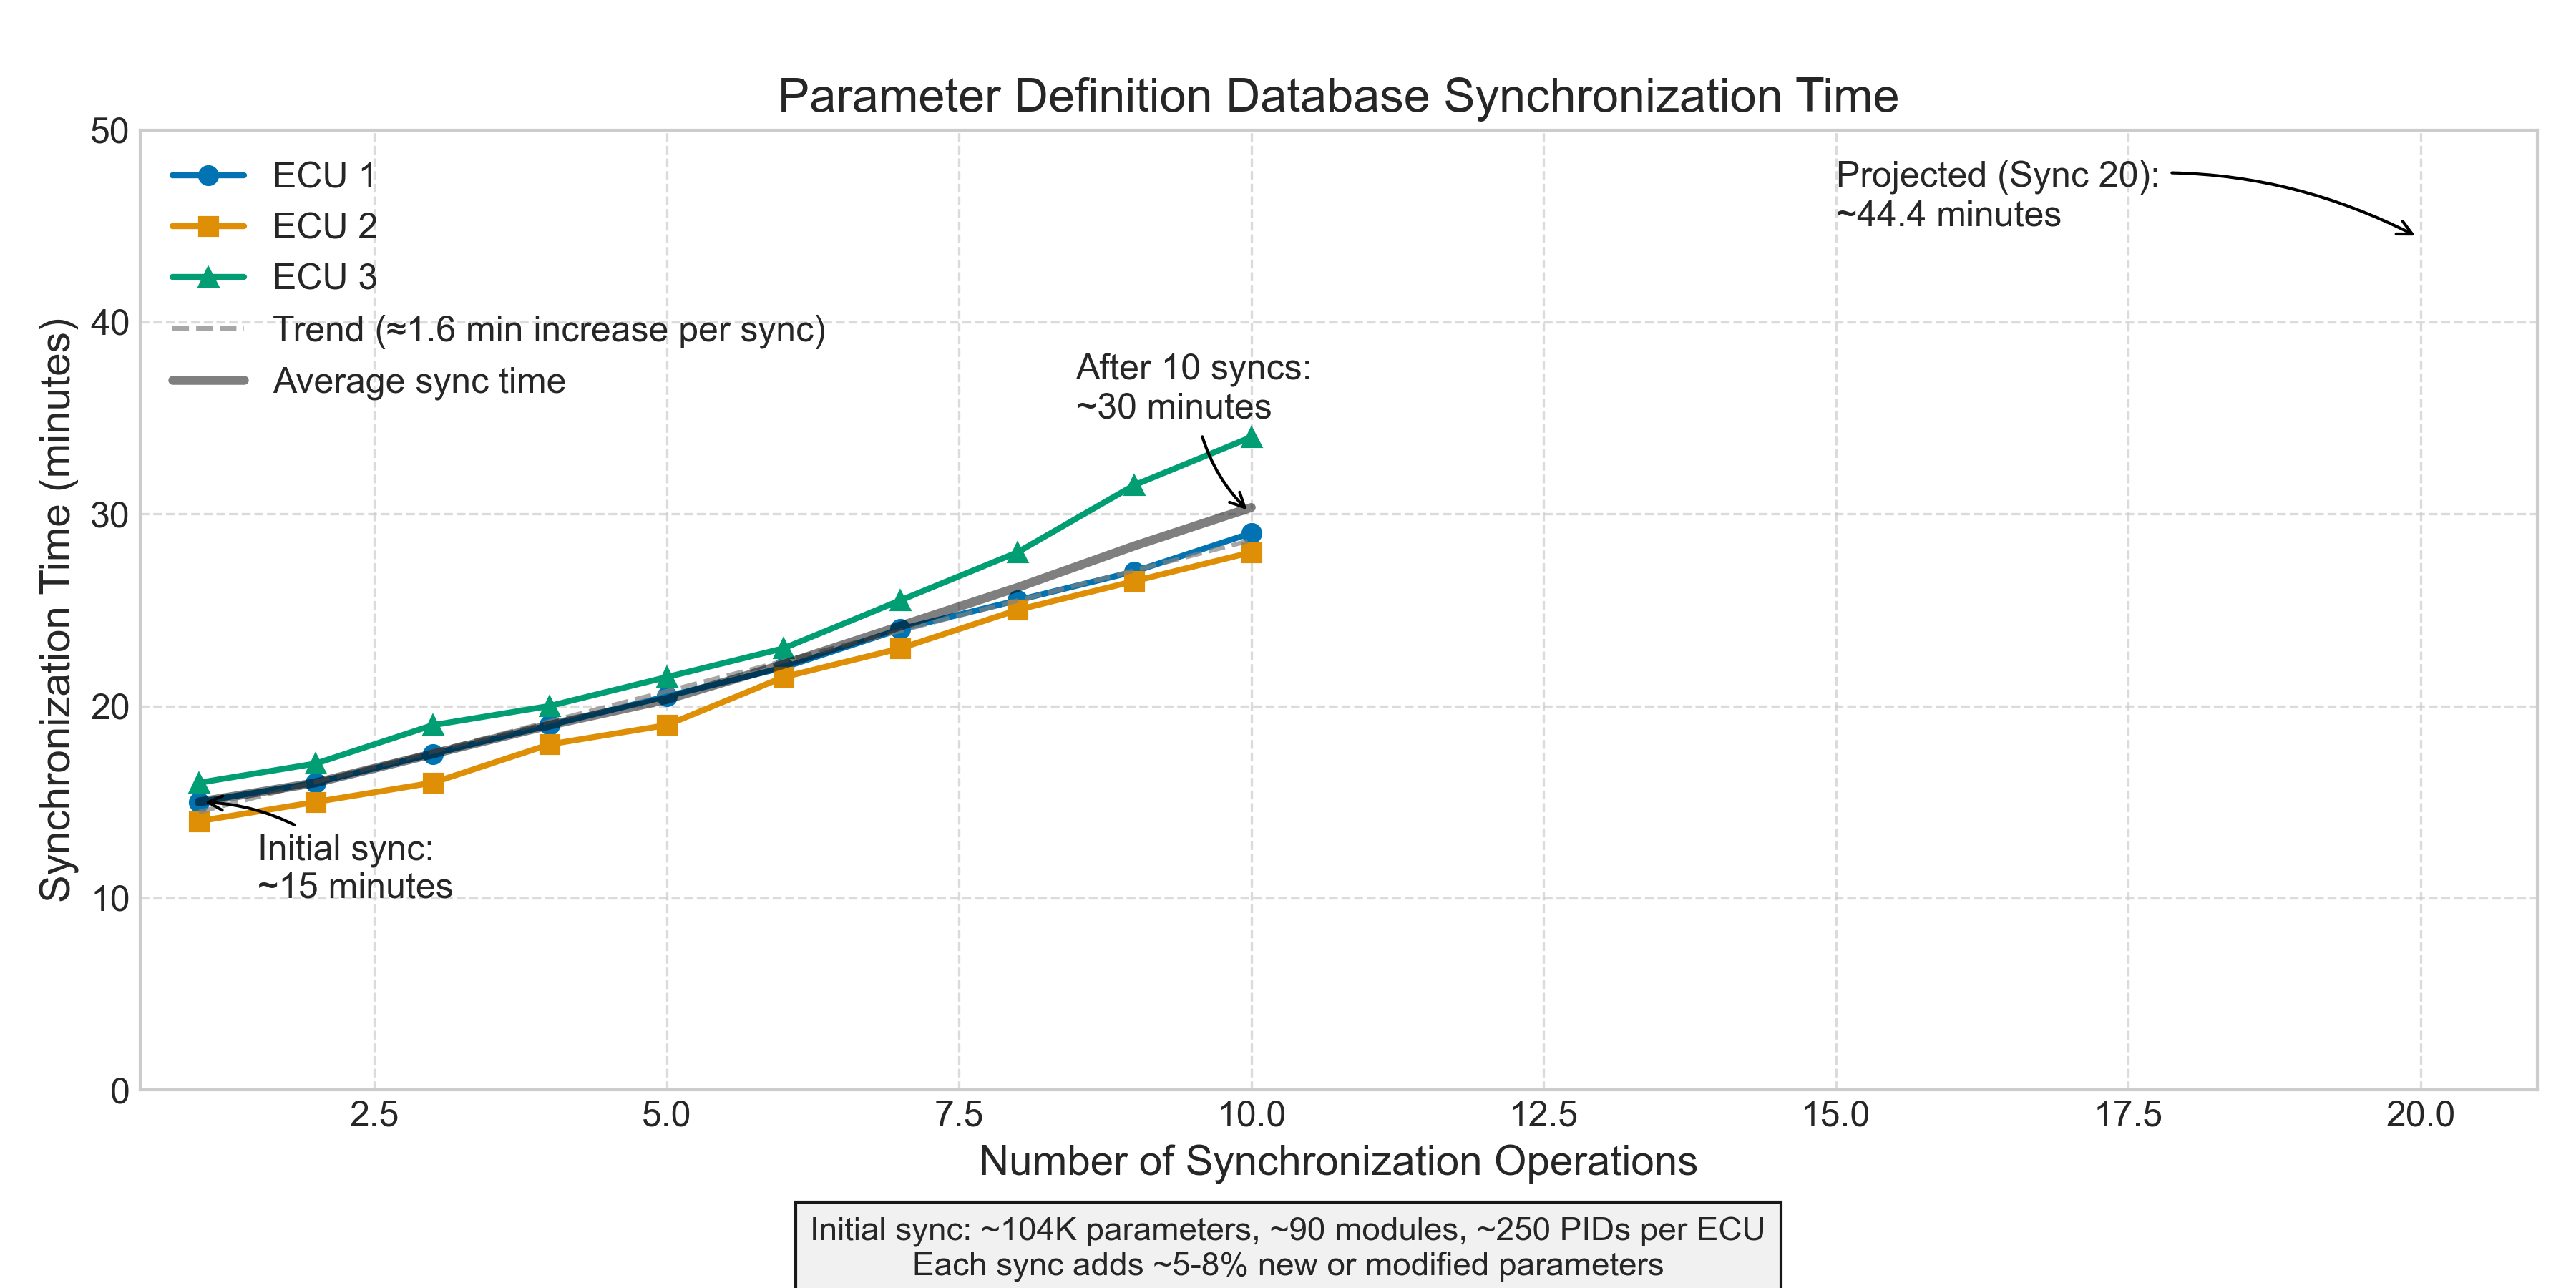
\includegraphics[width=0.8\textwidth]{figures/pdd_sync_time_graph.png}
    \caption{Parameter Definition Database Synchronization Time Trends}
    \label{fig:pdd-sync-time}
\end{figure}

The synchronization performance analysis revealed an increasing trend in execution time over successive synchronization operations. Initial synchronization operations required approximately 15 minutes for the tested \acp{ECU}, with execution times increasing to around 30 minutes after 10 synchronization cycles. This gradual increase aligns with the observations of Mueller and Müller \cite{mueller2018conception} regarding database synchronization in complex engineering environments.

Table \ref{tab:pdd-sync-results} presents the success rates for different types of parameter changes during synchronization operations.

\begin{table}[h]
\centering
\caption{Parameter Definition Database Synchronization Results}
\label{tab:pdd-sync-results}
\begin{tabular}{|l|c|c|c|}
\hline
\textbf{Change Type} & \textbf{Processed} & \textbf{Succeeded} & \textbf{Success Rate} \\
\hline
New Parameters & 5,218 & 5,218 & 100\% \\
\hline
Modified Parameters & 3,764 & 3,691 & 98.1\% \\
\hline
New Modules & 12 & 12 & 100\% \\
\hline
New \acp{PID} & 67 & 67 & 100\% \\
\hline
Removed Parameters & 42 & 42 & 100\% \\
\hline
\end{tabular}
\end{table}

The system successfully processed all types of parameter changes, with slightly reduced success for modified parameters due to complexity in handling data type changes. Based on the observed synchronization performance trends, the projected synchronization time for the 20th cycle would reach approximately 45 minutes. While still acceptable for the typical synchronization frequency, this suggests that synchronization performance optimization would be beneficial for long-term system maintenance.

Vehicle Configuration Database integration testing verified the system's ability to use vehicle configuration data for code rule evaluation and parameter file generation. Vehicle configuration data import testing confirmed that the system could correctly import and store vehicle configuration codes, with proper mapping between codes and vehicles. Code rule validation testing verified that the system could evaluate boolean expressions against vehicle configurations, with the evaluation engine correctly interpreting both simple logical operators and complex nested expressions. Parameter file generation testing confirmed that the system could produce valid parameter files for vehicle testing, with correct application of variant selection logic based on vehicle configuration codes.

\section{Feature Comparison with Excel-Based Approach}
\label{sec:feature-comparison-excel}

To assess the improvements provided by the \ac{VMAP} system, a feature comparison was conducted against the Excel-based approach currently used for parameter management. Table \ref{tab:feature-comparison} presents a comparison of key features between the \ac{VMAP} system and the Excel-based approach.

\begin{table}[h]
\centering
\caption{Feature Comparison with Excel-Based Approach}
\label{tab:feature-comparison}
\begin{tabular}{|l|c|c|}
\hline
\textbf{Feature} & \textbf{VMAP Database} & \textbf{Excel Approach} \\
\hline
Variant Management & Comprehensive & Limited \\
\hline
Multi-User Support & Concurrent & Sequential \\
\hline
Change Tracking & Automatic & Manual \\
\hline
Version Control & Phase-Based & File-Based \\
\hline
Access Control & Role + Module & File Permission \\
\hline
Validation & Automatic & Manual \\
\hline
Documentation & Integrated & Separate \\
\hline
Integration & Automated & Manual \\
\hline
\end{tabular}
\end{table}

The \ac{VMAP} system provides significant advantages in all feature categories, with particular improvements in multi-user support, change tracking, and access control. The \ac{VMAP} system demonstrated superior data integrity protection, correctly preventing invalid operations through database constraints and business rule validation. The database-level constraints and validation mechanisms provide a robust defense against data corruption, implementing the comprehensive validation approach described in Section \ref{sec:validation-mechanisms}.

Beyond technical improvements, the \ac{VMAP} system introduces significant enhancements to the automotive parameter development process. The centralized database approach enables concurrent work by multiple engineers, eliminating the file sharing bottlenecks common in the Excel-based approach. The role-based access control ensures that engineers can modify only their assigned modules, preventing accidental changes to other areas. The phase-based versioning approach aligns naturally with the automotive development lifecycle, supporting the structured progression from initial development through testing to final release. The comprehensive change tracking and documentation features address regulatory compliance requirements, providing complete traceability for all parameter modifications, increasingly important in the context of functional safety standards like ISO 26262.